%%%%%%%%%%%%%%%%%%%%%%%%%%%%%%%%%%%%%%%%%%%%%%%%
% E.Pinault-Bigeard - e.pinault-bigeard@upsti.fr
% http://s2i.pinault-bigeard.com
% CC BY-NC-SA 2.0 FR - http://creativecommons.org/licenses/by-nc-sa/2.0/fr/
%%%%%%%%%%%%%%%%%%%%%%%%%%%%%%%%%%%%%%%%%%%%%%%%
\documentclass[11pt]{article}
%%%%%%%%%%%%%%%%%%%%%%%%%%%%%%%%%%%%%%%%%%%%%%%%
% Package UPSTI_Document
%%%%%%%%%%%%%%%%%%%%%%%%%%%%%%%%%%%%%%%%%%%%%%%%
\usepackage{subcaption}
\usepackage{UPSTI_Document}
\usepackage{pgfplots}
\definecolor{darkspringgreen}{rgb}{0.09, 0.45, 0.27}

\newcommandx*{\dessinRepereFigGeo}[5][1=\vx{},2=\vy{},3=\vz{},4=,5=0]
	{
		\draw [->,very thick] (0,0) -- (1,0) ;
		\draw [->,very thick] (0,0) -- (0,1) ;
    \fill[white] (0,0) circle (0.13);
    \draw [->,very thick] (0,0) circle (0.13);
    \ifnumequal{#5}{0} {% z vers nous
      \fill[black] (0,0) circle (0.03);
      \draw [->,thick] (0,0) circle (0.04);
    }{% z vers la feuille
  		\begin{scope} [rotate=45]
  			\draw [-,thick] (0,-0.12) -- (0,0.12) ;
  			\draw [-,thick] (-0.12,0) -- (0.12,0) ;
  		\end{scope}
    }
		\draw [anchor=north west] (1.1,0) node {${#1}$};
		\draw [anchor=south west] (0,1.1) node {${#2}$};
		\draw [anchor=north east] (-0.1,0) node {${#3}$};
		\draw [anchor=north west] (-0.1,-0.1) node {${#4}$};
	}

%---------------------------------%
% Paramètres du package
%---------------------------------%

% Version du document (pour la compilation)
% 1: Document prof
% 2: Document élève
% 3: Document à publier
\newcommand{\UPSTIidVersionDocument}{1}

% Variante
%\newcommand{\UPSTIvariante}{2}

% Classe
% 1: PTSI				6: PSI*			11: TSI2		16: Spé
% 2: PT	(par défaut)	7: MPSI			12: ATS
% 3: PT*				8: MP			13: PC
% 4: PCSI				9: MP*			14: PC*
% 5: PSI				10: TSI1		15: Sup
%\newcommand{\UPSTIidClasse}{2}

% Affichage personnalisé de la classe
\newcommand{\UPSTIclasse}{Première STI2D}

% Matière
% 1: S2I (par défaut)    2: IPT     3: TIPE
%\newcommand{\UPSTIidMatiere}{9}

% Type de document
% 0: Custom*				7: Fiche Méthode			14: Document Réponses
% 1: Cours (par défaut)		8: Fiche Synthèse    		15: Programme de colle
% 2: TD     				9: Formulaire
% 3: TP						10: Memo
% 4: Colle					11: Dossier Technique
% 5: DS						12: Dossier Ressource
% 6: DM						13: Concours Blanc
% * Si on met la valeur 0, il faut décommenter la ligne suivante:
%\newcommand{\UPSTItypeDocument}{Custom}
\newcommand{\UPSTIidTypeDocument}{1}

% Titre dans l'en-tête
\newcommand{\UPSTItitreEnTete}{Modélisation du mouvement}
%\newcommand{\UPSTItitreEnTetePages}{UPSTItitreEnTetePages}
%\newcommand{\UPSTIsousTitreEnTete}{UPSTIsousTitreEnTete}

% Titre
\newcommand{\UPSTItitrePreambule}{Cinématique }
\newcommand{\UPSTItitre}{Mouvement, Vitesse, Accélération}

% Durée de l'activité (pour DS, DM et TP)
%\newcommand{\UPSTIduree}{3h}

% Note de bas de première page
%\newcommand{\UPSTInoteBasDePremierePage}{Note de bas de 1ère page}

% Numéro (ajoute " n°1" après DS ou DM)
%\newcommand{\UPSTInumero}{1}

% Numéro chapitre
\newcommand{\UPSTInumeroChapitre}{4}

% En-tête customisé
%\newcommand{\UPSTIenTetePrincipalCustom}{UPSTIenTetePrincipalCustom}

% Message sous le titre
%\newcommand{\UPSTImessage}{Message sous le titre}

% Référence au programme
%\newcommand{\UPSTIprogramme}{\EPBComp \EPBCompP{B1-02}, \EPBCompP{B2-49}, \EPBCompS{B2-50}, \EPBCompS{B2-51}, \EPBCompP{C1-07}, \EPBCompP{C1-08}}

% Si l'auteur n'est pas l'auteur par défaut
%\renewcommand{\UPSTIauteur}{UPSTI}

% Si le document est réalisé au nom de l'équipe
%\newcommand{\UPSTIdocumentCollegial}{1}

% Source
%\newcommand{\UPSTIsource}{UPSTI}

% Version du document
\newcommand{\UPSTInumeroVersion}{1.0}

%-----------------------------------------------
\UPSTIcompileVars		% "Compile" les variables
%%%%%%%%%%%%%%%%%%%%%%%%%%%%%%%%%%%%%%%%%%%%%%%%


%%%%%%%%%%%%%%%%%%%%%%%%%%%%%%%%%%%%%%%%%%%%%%%%
% Début du document
%%%%%%%%%%%%%%%%%%%%%%%%%%%%%%%%%%%%%%%%%%%%%%%%
\begin{document}
\UPSTIbuildPage

\UPSTIobjectif{Dans ce cours, nous nous intéresserons à l'analyse des positions, de la vitesse et de l'accélération d'un point et d'une pièce (ou plus généralement un objet en mouvement). L’analyse des grandeurs cinématiques (position, vitesse et accélération) permet de prévoir la géométrie et les dimensions de pièces, de composants. }

\section{Introduction}

\UPSTIdefinition{{La cinématique est la partie de la mécanique qui permet d’étudier et de décrire les mouvements des corps, d’un point de vue purement mathématique, indépendamment des causes qui les produisent.}}

\section{Hypothèse}
Comme n'importe quel modélisation du réel, la cinématique considère certaines hypothèses.

L'hypothèse principale faite en cinématique est que l'on \textbf{considère les solides comme étant indéformables}.
\UPSTIrappel[Solide indéformable]{

\begin{UPSTIaCompleterEnv}
  Une pièce mécanique \solide{S} peut être considérée comme un solide indéformable si quels que soient les points $C$ et $B$ appartenant à \solide{S} la distance $CB$ reste constante au cours du temps.
\end{UPSTIaCompleterEnv}

\UPSTIeleveOnly{\UPSTIpointilles}
}



\pagebreak
\section{Trajectoire d'un point}
\subsection{Référentiel et repère}

\begin{UPSTIactivite}
\begin{center}
  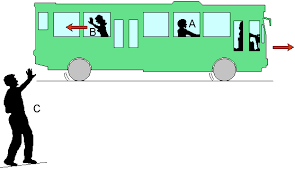
\includegraphics[width=.4\textwidth]{Src/Images/bus_mouvement_relatif}
\end{center}

Imaginons qu'une personne $B$ soit dans un bus (voir figure ci-dessus). Elle se déplace de l'avant vers l'arrière du bus. Une personne $A$ est assise dans le train, elle regarde dans le sens de la marche.
\UPSTIquestion{Par rapport à $A$, comment se déplace $B$ ? (Va-t-elle vers l'arrière, vers l'avant ou est-elle immobile ?)}

\UPSTIeleveOnly{\UPSTIpointilles[1]}
\UPSTIcorrection{Pour A, B se déplace vers l'arrière.}
\UPSTIquestion{Pour $A$, cette personne va-t-elle lentement ou rapidement ?}

\UPSTIeleveOnly{\UPSTIpointilles[1]}
\UPSTIcorrection{Pour A, B se déplace lentement.}
\UPSTIquestion{Une personne $C$ est sur le bord de la voie. Elle voit passer le train. Par rapport à $C$, comment se déplace $A$ ? Se déplace-t-elle rapidement ?}

\UPSTIeleveOnly{\UPSTIpointilles[1]}
\UPSTIcorrection{Pour C, B se déplace \textbf{rapidement} vers l'avant.}

\end{UPSTIactivite}

On le voit dans cet exemple, la trajectoire d'un point n'est pas la même selon le point de vue que l'on considère. Ainsi, il est \textbf{impératif} de préciser par rapport à quoi on s'exprime lorsque l'on caractérise un mouvement.

\UPSTIaRetenir{
\begin{itemize}
  \item Afin d'étudier le mouvement d'un point ou d'un système de solides, il est nécessaire de mettre en place un système de référence appelé \textit{référentiel}. Il représente en quelque sorte la position d'observation des phénomènes.
  \item Un repère est défini par une origine $O$ et trois vecteurs orthonormés directs \bxyz. Il se note \rROxyz
  \item La \UPSTIfig{fig:reperes} représente le repère direct \rROxyz vu de différents points de vues.
\end{itemize}
}

\begin{figure}[!ht]
  \centering
  \begin{subfigure}[b]{.3\textwidth}
    \centering
    \dessinRepere[\vx{}][\vy{}][\vz{}][O]
    \caption{\vz{} vers nous}
  \end{subfigure}
  \begin{subfigure}[b]{.3\textwidth}
    \centering
    \dessinRepere[\vz{}][\vx{}][\vy{}][O]
    \caption{\vy{} vers nous}
  \end{subfigure}
  \begin{subfigure}[b]{.3\textwidth}
    \centering
    \dessinRepere[\vy{}][\vz{}][\vx{}][O]
    \caption{\vx{} vers nous}
  \end{subfigure}
  \caption{Le repère \rROxyz}
  \label{fig:reperes}
\end{figure}
\pagebreak


\begin{UPSTIactivite}
  Pour décrire la position d'un point dans un repère, on utilise ses coordonnées par rapport au centre du repère.

    \begin{center}
      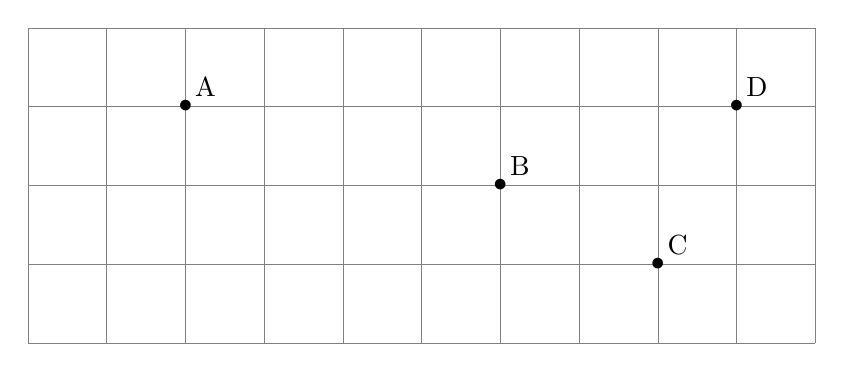
\begin{tikzpicture}
        \draw [very thin, gray] (0,0) grid (10,4);
        \dessinRepereFigGeo[\vx{}][\vy{}][\vz{}][O]
        \begin{scope}[shift={(4,2)}]
          \dessinRepereFigGeo[\vy{1}][\vz{1}][\vx{1}][G]
        \end{scope}
        \draw (2,3) node{$\bullet$} node[above right]{A};
        \draw (6,2) node{$\bullet$} node[above right]{B};
        \draw (8,1) node{$\bullet$} node[above right]{C};
        \UPSTIprofOnly{\draw (9,3) node{$\bullet$} node[above right]{D};}
      \end{tikzpicture}
    \end{center}

    \UPSTIexemple{Le point $C$ a pour coordonnées $(8,1,0)$ dans le repère \rROxyz. Le point $C$ a pour coordonnées $(0,4,-1)$ dans le repère \repere[\rR{1}]{G}{\vx{1}}{\vy{1}}{\vz{1}}.}

  \resetNumQuestion
  % ----- Question ------
  \UPSTIquestion{Donner les coordonnées des points A et B dans le repère \rROxyz}

  \UPSTIeleveOnly{\UPSTIpointilles[1]}

  \UPSTIcorrection{ Dans \rROxyz : $A(2,3,0)$ et $B(6,2,0)$.}

  % ----- Question ------
  \UPSTIquestion{Donner les coordonnées des point A et B dans le repère \repere[\rR{1}]{G}{\vx{1}}{\vy{1}}{\vz{1}} }

  \UPSTIeleveOnly{\UPSTIpointilles[1]}

  \UPSTIcorrection{ Dans \repere[\rR{1}]{G}{\vx{1}}{\vy{1}}{\vz{1}} : $A(0,-2,1)$ et $B(0,2,0)$.}

  \UPSTIquestion{Placer le point $D$ de coordonnées $(0,5,1)$ dans le repère \repere[\rR{1}]{G}{\vx{1}}{\vy{1}}{\vz{1}}}

  \resetNumQuestion
\end{UPSTIactivite}

\subsection{Trajectoire}
\UPSTIdefinition{On appelle trajectoire du point ($M$) d’un solide \solide{S} l’ensemble des positions occupées successivement par ce point, au cours du temps, lors son déplacement par rapport à un référentiel donné. \\
La trajectoire du point $M$ appartenant à \solide{S} par rapport au repère \rR{} se note \trajectoire{M}{S}{R}}

\UPSTIexemple[Trajectoire de la pointe d'un stylo]{
La trajectoire de la pointe du stylo par rapport à la feuille est la trace laissée par cette pointe sur la feuille.

}

\subsubsection{Différents types de trajectoires}
\UPSTIaRetenir{On pourra différentier trois grands types de trajectoires pour un point :

\UPSTIeleveOnly{\UPSTIpointilles}

\UPSTIprofOnly{
  \begin{itemize}
    \item La droite
    \item L'arc de cercle (ou le cercle complet)
    \item Une trajectoire quelconque
  \end{itemize}}
}

\begin{figure}[!ht]
  \centering
  \begin{subfigure}[b]{.3\textwidth}
    \centering
    \begin{tikzpicture}
      \draw (0,0) -- (2,1);
    \end{tikzpicture}
    \caption{Trajectoire droite}
  \end{subfigure}
  \begin{subfigure}[b]{.3\textwidth}
    \centering
    \begin{tikzpicture}
      \draw (1,0) arc (10:170:1) ;
    \end{tikzpicture}
    \caption{Trajectoire circulaire}
  \end{subfigure}
  \begin{subfigure}[b]{.3\textwidth}
    \centering
      \begin{tikzpicture}
        \draw plot [domain=-0.8:0.8] (\x,\x^2);
      \end{tikzpicture}
    \caption{Trajectoire curviligne.}
  \end{subfigure}
  \caption{Différents types de trajectoires.}
  \label{fig:diff_traj}
\end{figure}

\subsection{Vitesse et vecteur vitesse}
Une trajectoire ne suffit pas pour déterminer le mouvement d'un point dans un repère. En effet, cette trajectoire peut-être faite de manière rapide ou lente. La rapidité ou la lenteur est représentée par la vitesse du point.

\UPSTIaRetenir{
La vitesse d'un point est représentée par
\begin{itemize}
  \item de direction tangente à la trajectoire du UPSTIpointilles
  \item de même sens que la trajectoire du point
  \item de norme égale au déplacement divisé par la durée du déplacement
\end{itemize}

  La vitesse moyenne d'un point $M$ se déplaçant de $M(t_1)$ à $M(t_2)$ est de \UPSTIcadreMath{\norme{\vVitesse{M}{}{}} = \frac{M(t_1)M(t_2)}{t_2-t_1}}.

  En écrivant $d$ la distance $d = M(t_1)M(t_2)$ et avec $\Delta t = t_2-t_1$, on a \UPSTIcadreMath{\norme{\vVitesse{M}{}{}} = \frac{M(t_1)M(t_2)}{t_2-t_1} =  \huge{\frac{d}{\Delta t}}}

  La vitesse s'exprime en \si{m/s}.
}

\begin{figure}
  \centering
  \begin{tikzpicture}
  \path(0 ,0)coordinate(A);
  \path(3 ,3)coordinate(B);
  \path(8 ,0)coordinate(C);
  \path(1 ,1)coordinate(ctrl1);
  \path(0 ,3)coordinate(ctrl2);
  \path(6 ,3)coordinate(ctrl3);
  \path(6 ,0)coordinate(ctrl4);
  \draw(A)  .. controls(ctrl1)and(ctrl2)  ..  (B) .. controls(ctrl3)and(ctrl4) .. (C);%
  \draw[->,red,very thick] (B) -- (ctrl3) node[near end, above] {\vVitesse{B}{}{0}};;
  \draw[red] (B) node{$\bullet$} node[above]{B};
  \draw[->,blue,very thick] (A) -- (ctrl1) node[near end, below right] {\vVitesse{A}{}{0}};
  \draw[blue] (A) node{$\bullet$} node[below]{A};
\end{tikzpicture}

  \caption{La vitesse d'un point est tangeante à la trajectoire}
  \label{fig:exemple}
\end{figure}

\UPSTIattention{La vitesse d'un point est un \textbf{vecteur}. Elle a donc une composante sur \vx{}, sur\vy{} et sur \vz{}.}


\begin{UPSTIactivite}
  \begin{center}
    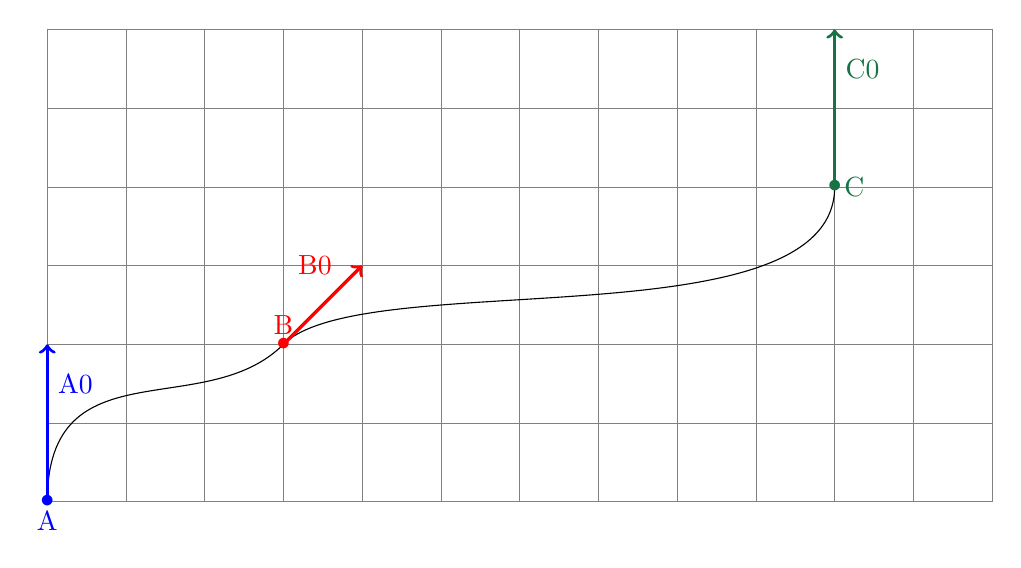
\begin{tikzpicture}
  \draw [very thin, gray] (0,0) grid (12,6);
  \path(0 ,0)coordinate(A);
  \path(3 ,2)coordinate(B);
  \path(10 ,4)coordinate(C);
  \path(0 ,2)coordinate(ctrl1);
  \path(2 ,1)coordinate(ctrl2);
  \path(4 ,3)coordinate(ctrl3);
  \path(10 ,2)coordinate(ctrl4);
  \path(10, 6)coordinate(ctrl5);
  \draw(A)  .. controls(ctrl1)and(ctrl2)  ..  (B) .. controls(ctrl3)and(ctrl4) .. (C);%
  \UPSTIprofOnly{\draw[->,red,very thick] (B) -- (ctrl3) node[near end, above left] {\vVitesse{B}{}{0}};}
  \draw[red] (B) node{$\bullet$} node[above]{B};
  \UPSTIprofOnly{\draw[->,blue,very thick] (A) -- (ctrl1) node[near end, right] {\vVitesse{A}{}{0}};}
  \draw[blue] (A) node{$\bullet$} node[below]{A};
  \UPSTIprofOnly{\draw[->,darkspringgreen,very thick] (C) -- (ctrl5) node[near end, right] {\vVitesse{C}{}{0}};}
  \draw[darkspringgreen] (C) node{$\bullet$} node[right]{C};
\end{tikzpicture}

  \end{center}
  \UPSTIquestion{Tracer l'allure des vecteurs vitesses des points A, B et C}
\end{UPSTIactivite}


\subsection{Accélération - Variation de vitesse}
Nous venons de voir que la vitesse moyenne représente la variation de la position sur un intervalle de temps. De la même façon, l'accélération modélise la variation de vitesse sur un intervalle de temps.

\UPSTIaRetenir{
L'accélération correspond à la variation de vitesse entre deux instants :
\UPSTIcadreMath{a = \frac{v(t_2)-v(t_1)}{t_2-t_1}=\frac{\Delta v}{\Delta t}}, avec $v(t_i)$ la norme de la vitesse à l'instant $t_i$.

L'accélération s'exprime en $m/s^2$.
}

\UPSTIaRetenir{
Lorsque la vitesse est constante, l'accélération est nulle.
}

\begin{UPSTIactivite}
  \resetNumQuestion
  \begin{center}
    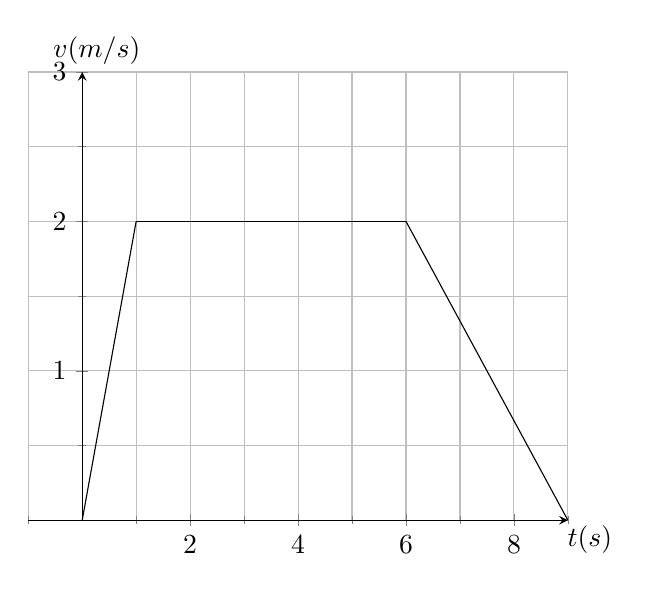
\begin{tikzpicture}
  \begin{axis}[grid=both,%
    %axis x line=center,%
  %axis y line=center,%
    ymin=0,ymax=3,xmax=9,xmin=-1,%
    %xticklabel=\empty,%
    %yticklabel=\empty, %
    minor tick num=1,axis lines = middle,xlabel=$t(\si{s})$,ylabel=$v(\si{m/s})$,label style =
               {at={(ticklabel cs:1.1)}}]
    \addplot [mark=none,domain=0:1] {2*x};
    \addplot [mark=none,domain=1:6] {2};
    \addplot [mark=none,domain=6:9] {6 -2*x/3};
  \end{axis}
  % \draw [very thin, gray] (0,0) grid (12,4);
  % \path(0 ,0)coordinate(A);
  % \path(3 ,2)coordinate(B);
  % \path(10 ,4)coordinate(C);
  % \path(0 ,2)coordinate(ctrl1);
  % \path(2 ,1)coordinate(ctrl2);
  % \path(4 ,3)coordinate(ctrl3);
  % \path(10 ,2)coordinate(ctrl4);
  % \path(10, 6)coordinate(ctrl5);
  % \draw(A)  .. controls(ctrl1)and(ctrl2)  ..  (B) .. controls(ctrl3)and(ctrl4) .. (C);%
  % \UPSTIprofOnly{\draw[->,red,very thick] (B) -- (ctrl3) node[near end, above] {\vVitesse{B}{}{0}};}
  % \draw[red] (B) node{$\bullet$} node[above]{B};
  % \UPSTIprofOnly{\draw[->,blue,very thick] (A) -- (ctrl1) node[near end, below right] {\vVitesse{A}{}{0}};}
  % \draw[blue] (A) node{$\bullet$} node[below]{A};
  % \UPSTIprofOnly{\draw[->,blue,very thick] (C) -- (ctrl5) node[near end, below right] {\vVitesse{C}{}{0}};}
  % \draw[darkspringgreen] (C) node{$\bullet$} node[right]{C};
\end{tikzpicture}

  \end{center}

  \UPSTIquestion{Sur le graph, identifier trois phase de mouvement différentes.}

  \UPSTIquestion{Calculer l'accélération moyenne entre $t=\SI{0}{s}$ et $t=\SI{1}{s}$. }

  \UPSTIeleveOnly{\UPSTIpointilles}

  \UPSTIcorrection{$a=\frac{\Delta v}{\Delta t} = \frac{2}{1} = \SI{2}{m/s^2}$}

  \UPSTIquestion{Calculer l'accélération moyenne entre $t=\SI{1}{s}$ et $t=\SI{6}{s}$. }

  \UPSTIeleveOnly{\UPSTIpointilles}

  \UPSTIcorrection{$a=\frac{\Delta v}{\Delta t} = \frac{0}{1} = \SI{0}{m/s^2}$}

  \UPSTIquestion{Calculer l'accélération moyenne entre $t=\SI{6}{s}$ et $t=\SI{9}{s}$. }

  \UPSTIeleveOnly{\UPSTIpointilles}

  \UPSTIcorrection{$a=\frac{\Delta v}{\Delta t} = \frac{2}{3} = \SI{-0,66}{m/s^2}$}
  \resetNumQuestion
\end{UPSTIactivite}


\pagebreak
\section{Différents types de mouvements}
\subsection{Translations}
\UPSTIdefinition[Mouvement de Translation]{Un solide est en mouvement de translation lorsqu'un
segment quelconque de ce solide reste parallèle à lui-même au cours du déplacement.}

%\UPSTIremarque{
Cela revient à dire que lorsqu'un solide est en translation, toutes les photos prises de cet objet au cours du temps seraient identiques
%}

\subsubsection{Translation rectiligne}
\UPSTIexemple[Une voiture en ligne droite]{
  La voiture de la \UPSTIfig{fig:rectiligne} est translation rectiligne.
  \begin{figure}[!ht]
    \centering
    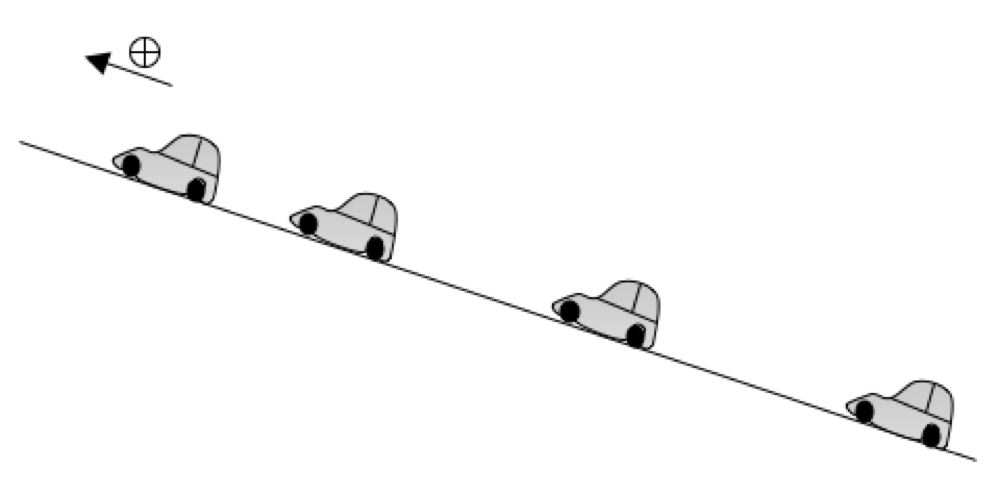
\includegraphics[width=.4\textwidth]{Src/Images/voiture_translation}
    \caption{Translation rectiligne}
    \label{fig:rectiligne}
  \end{figure}
}

\UPSTIaRetenir{Une translation est dite \textbf{rectiligne} lorsque les trajectoires des points du solides sont des \textbf{segments} (ou droites).}

\UPSTIaRetenir{La translation rectiligne uniforme désigne un mouvement de translation en \textbf{ligne droite} et à \textbf{vitesse constante}.}

\begin{UPSTIactivite}
  Soit une voiture en translation rectiligne uniforme de vitesse $v=\SI{15}{m/s}$.
  \UPSTIquestion{Calculer la distance parcourue en \SI{20}{min}}

  \UPSTIeleveOnly{\UPSTIpointilles}

   \begin{UPSTIcorrectionEnv}{

     On a $v=\SI{15}{m/s}$. On sait que $v=\frac{d}{\Delta t}$. On a donc $d=v\times\Delta t = 15 \times 20\times 60 = \SI{18000}{m} = \SI{18}{km}$ }
   \end{UPSTIcorrectionEnv}

  \UPSTIquestion{Que vaut l'accélération de cette voiture ?}

  \UPSTIeleveOnly{\UPSTIpointilles}
\begin{UPSTIcorrectionEnv}{

  La vitesse étant constante, l'accélération est nulle.}
\end{UPSTIcorrectionEnv}
\end{UPSTIactivite}


\subsubsection{Translation circulaire}
\UPSTIexemple[Une cabine de grande roue]{
  La cabine supendue à la grande roue de la \UPSTIfig{fig:circulaire} est translation circulaire.
  \begin{figure}[!ht]
    \centering
    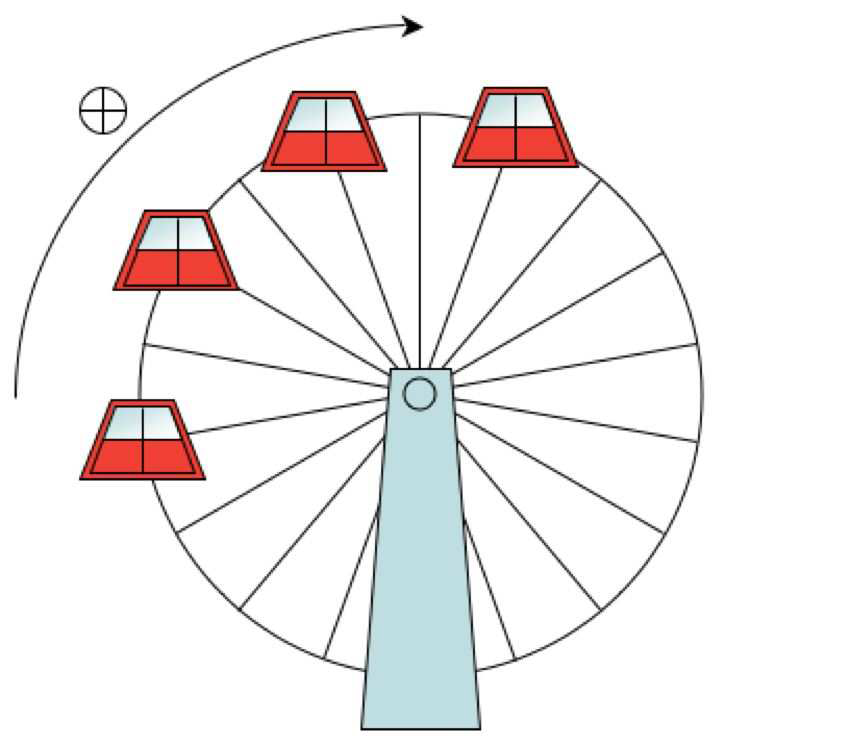
\includegraphics[width=.4\textwidth]{Src/Images/translation_circulaire_manege}
    \caption{Translation circulaire}
    \label{fig:circulaire}
  \end{figure}}
  \UPSTIaRetenir{Une translation est dite \textbf{circulaire} lorsque les trajectoires des points du solides sont des \textbf{cercles}.}

  \UPSTIattention{La grande roue est en rotation, c'est bien la \textbf{cabine} qui est en translation ciruclaire car elle se déplace sans tourner par rapport au sol}


\subsubsection{Translation curviligne}
\UPSTIexemple[Une cabine de téléphérique]{
  La cabine du téléphérique de la \UPSTIfig{fig:curviligne} est translation curviligne.
  \begin{figure}[h!t]
    \centering
    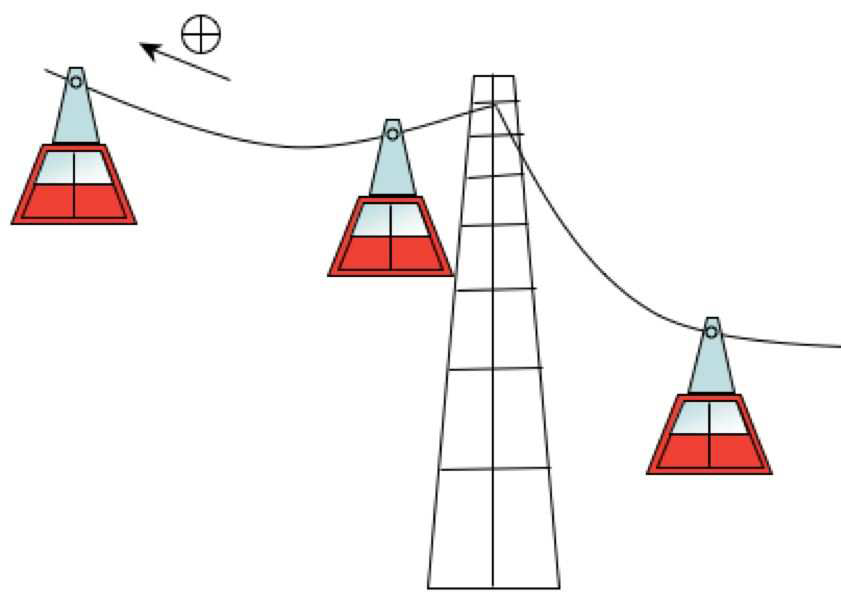
\includegraphics[width=.35\textwidth]{Src/Images/translation_curviligne_telesiege}
    \caption{Translation curviligne}
    \label{fig:curviligne}
  \end{figure}
}

\UPSTIaRetenir{Une translation est dite \textbf{curviligne} lorsque les trajectoires des points du solides sont des \textbf{courbe}. C'est à dire lorsqu'il s'agit d'une translation qui n'est ni rectiligne, ni circulaire.}

\subsection{Rotation}
\UPSTIexemple[Une bouteille de lait que l'on fait tourner]{
La bouteille de lait de la \UPSTIfig{fig:rotation} est en rotation.
\begin{figure}[h!t]
  \centering
  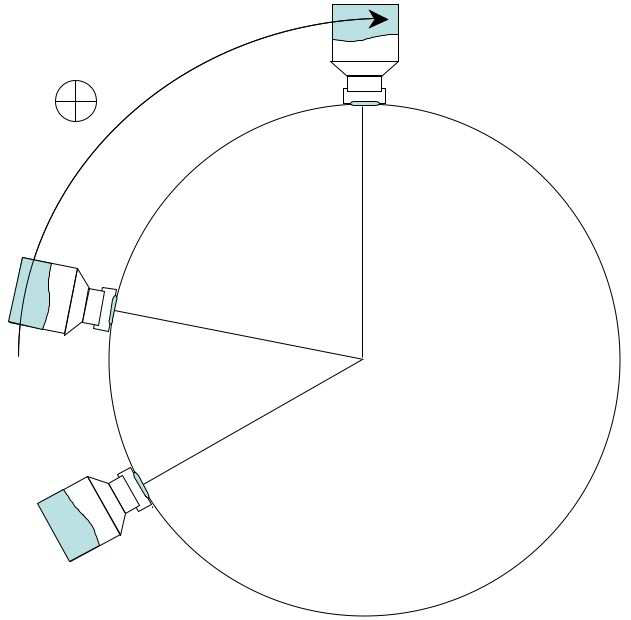
\includegraphics[width=.4\textwidth]{Src/Images/rotation_lait}
  \caption{Rotation}
  \label{fig:rotation}
\end{figure}
}
\UPSTIdefinition{Un solide est en mouvement de rotation lorsque tout point de ce solide reste à une distance fixe du centre de rotation. Cela veut dire que tous les points du solide se déplacent sur des cercles qui ont un même centre.}




\end{document}
